\documentclass[10pt]{article}

% Packages
\usepackage{graphicx}
\usepackage{a4wide}
\usepackage{amsfonts}
\usepackage{amssymb}
\usepackage{amsmath}
\usepackage{anslistings}

% Geometry
\usepackage[left=15mm,top=27mm,bottom=27mm,right=15mm]{geometry}

% Commands
\newcommand{\dx}{\,\mathrm{d}x}
\DeclareMathOperator{\grad}{\mathrm{grad}}

\pagestyle{empty}

\begin{document}

\null
\vspace{-2.5cm}

\begin{center}
  \bf
  \LARGE
  Solving Partial Differential Equations in Python

  \bigskip

  \emph{--- Finite element methods and FEniCS programming ---}

  \bigskip

  \Large
  Beijing Institute for Scientific and Engineering Computing (BISEC)

  \smallskip

  August 3--6 2015


\end{center}

\smallskip

\begin{center}
  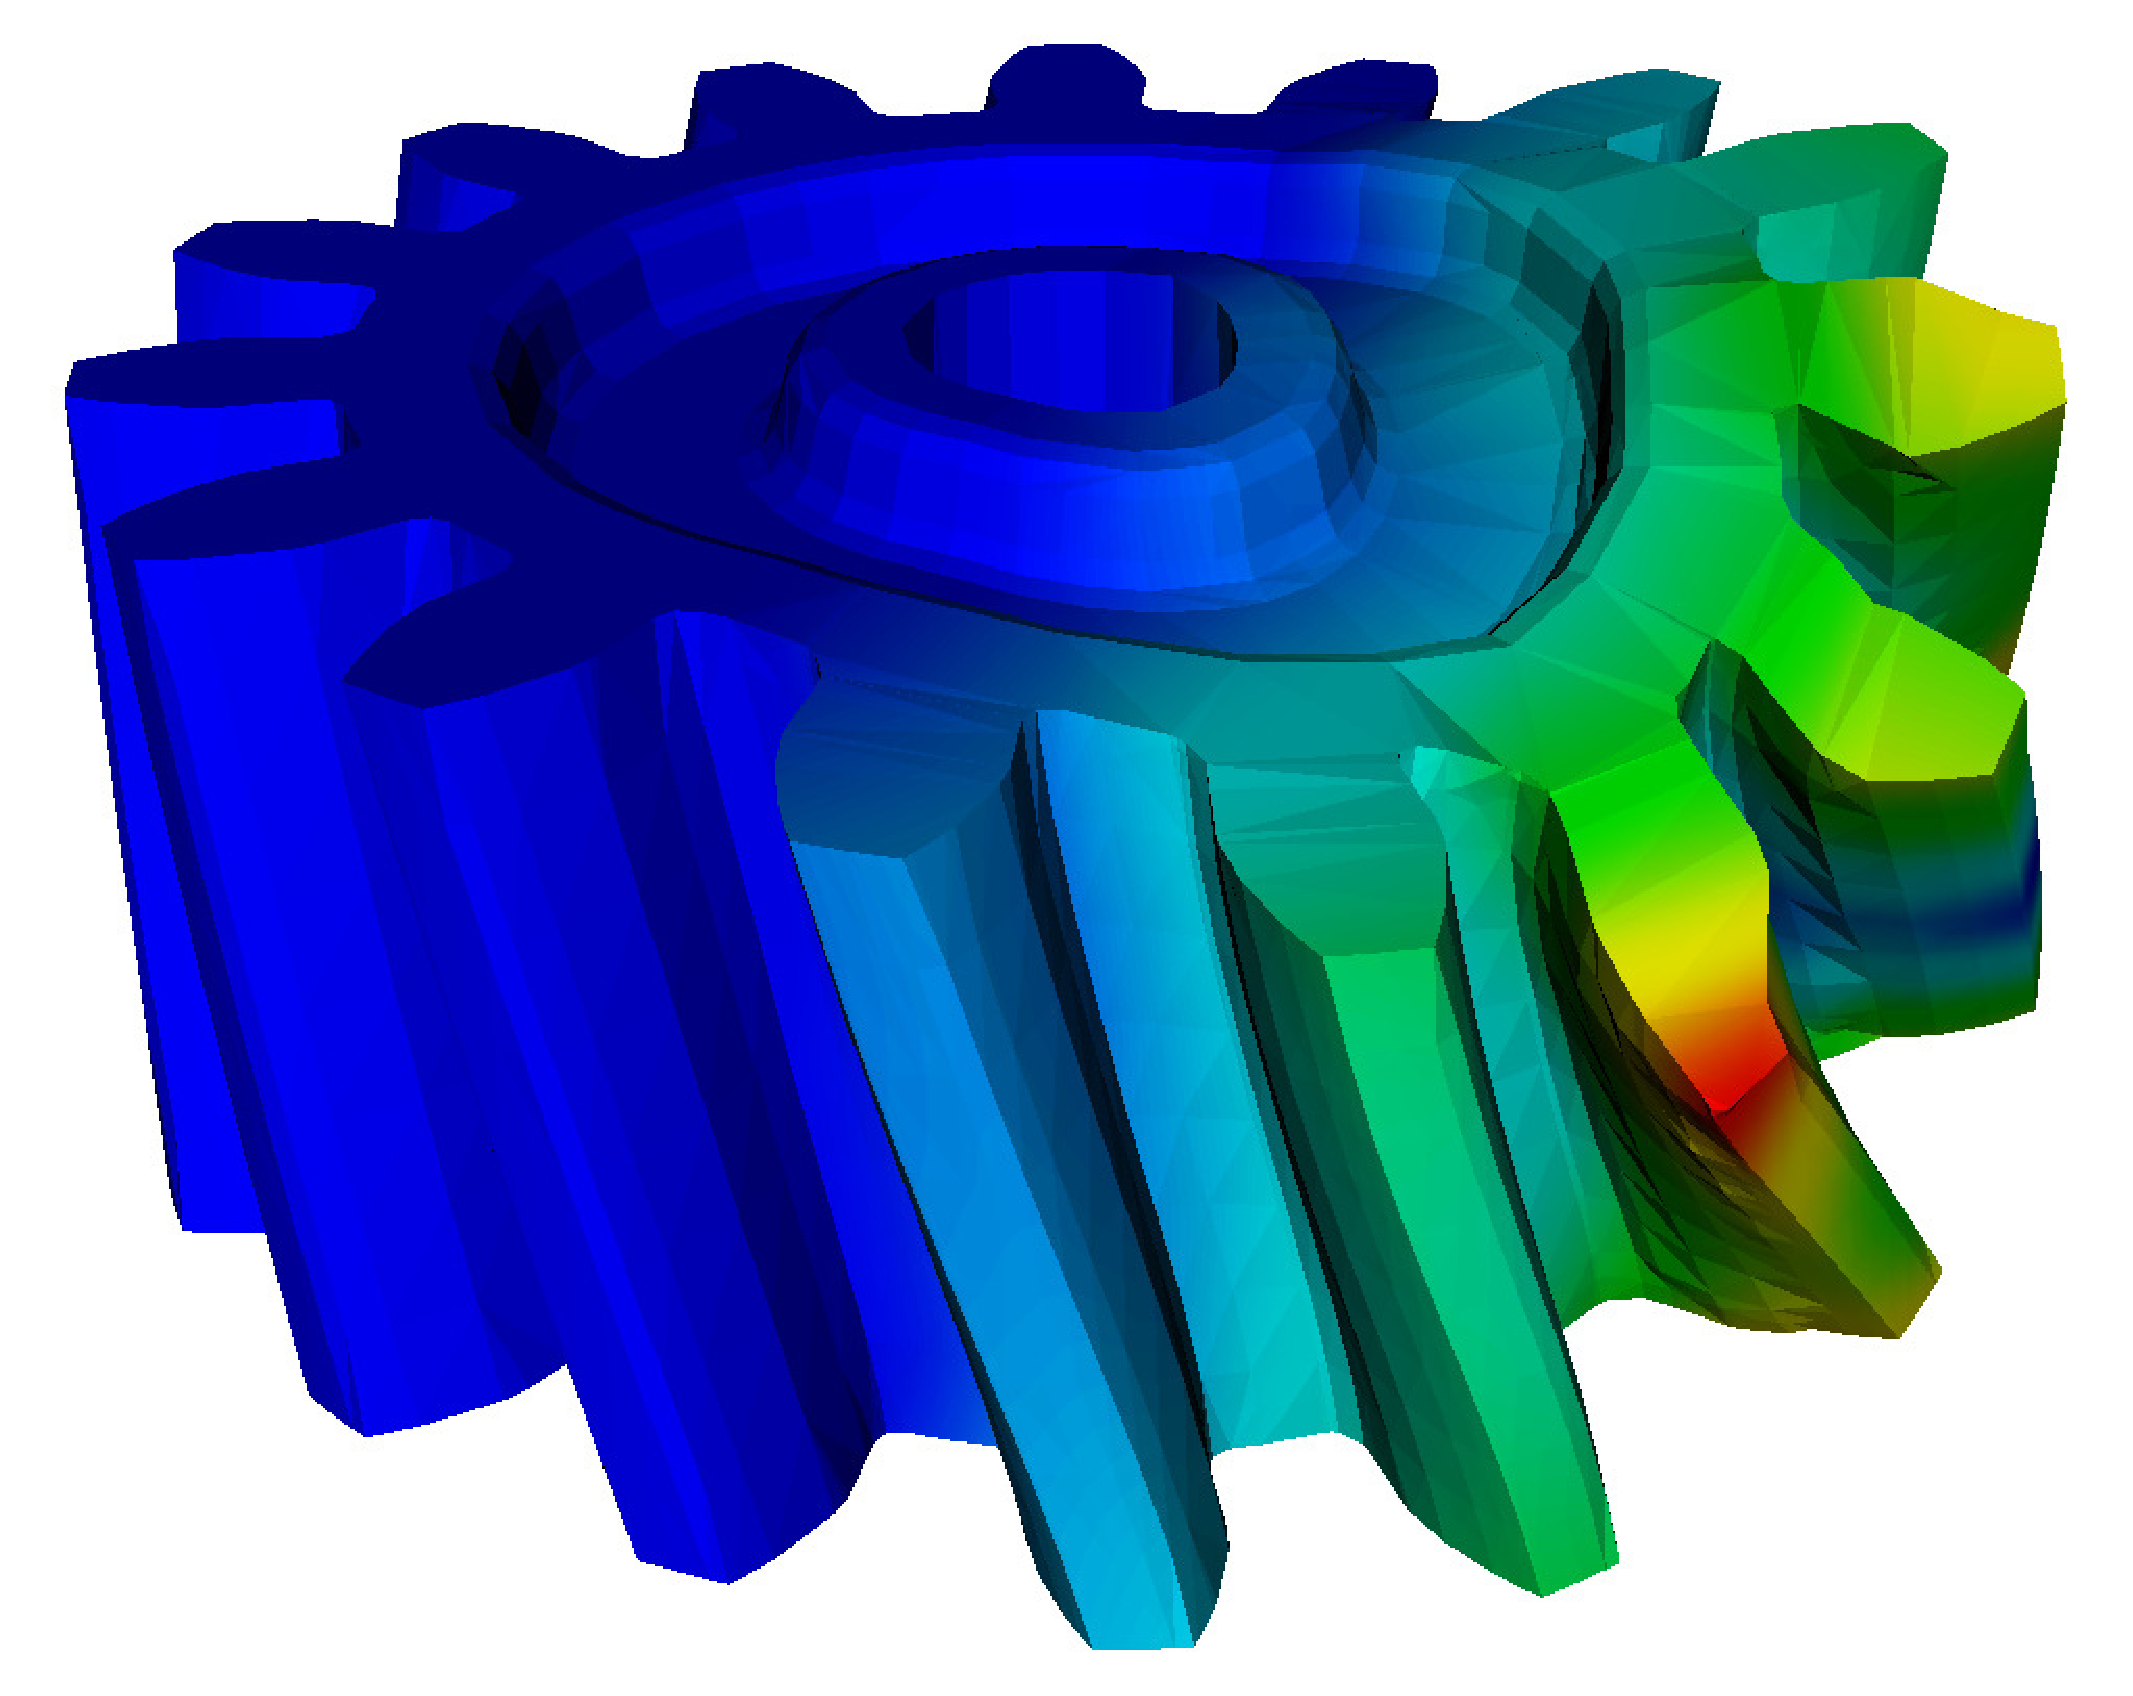
\includegraphics[height=2.5cm]{pdf/elasticity.pdf}
  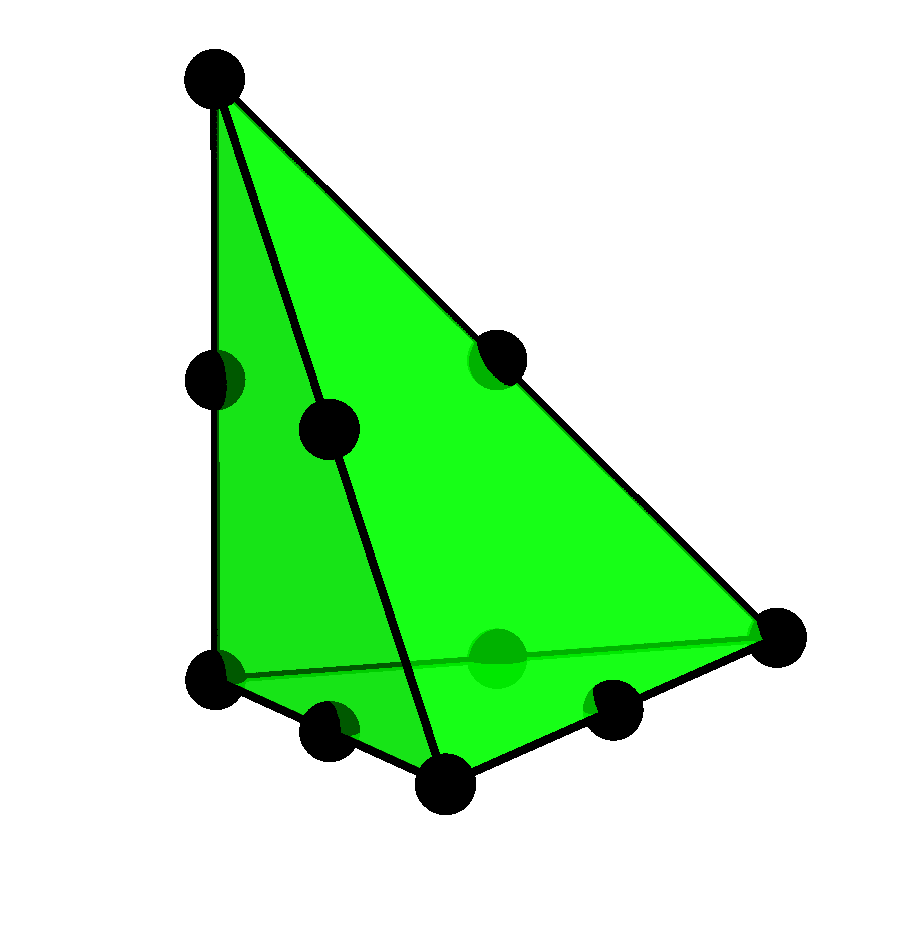
\includegraphics[height=2.5cm]{png/CG2_3d.png}
  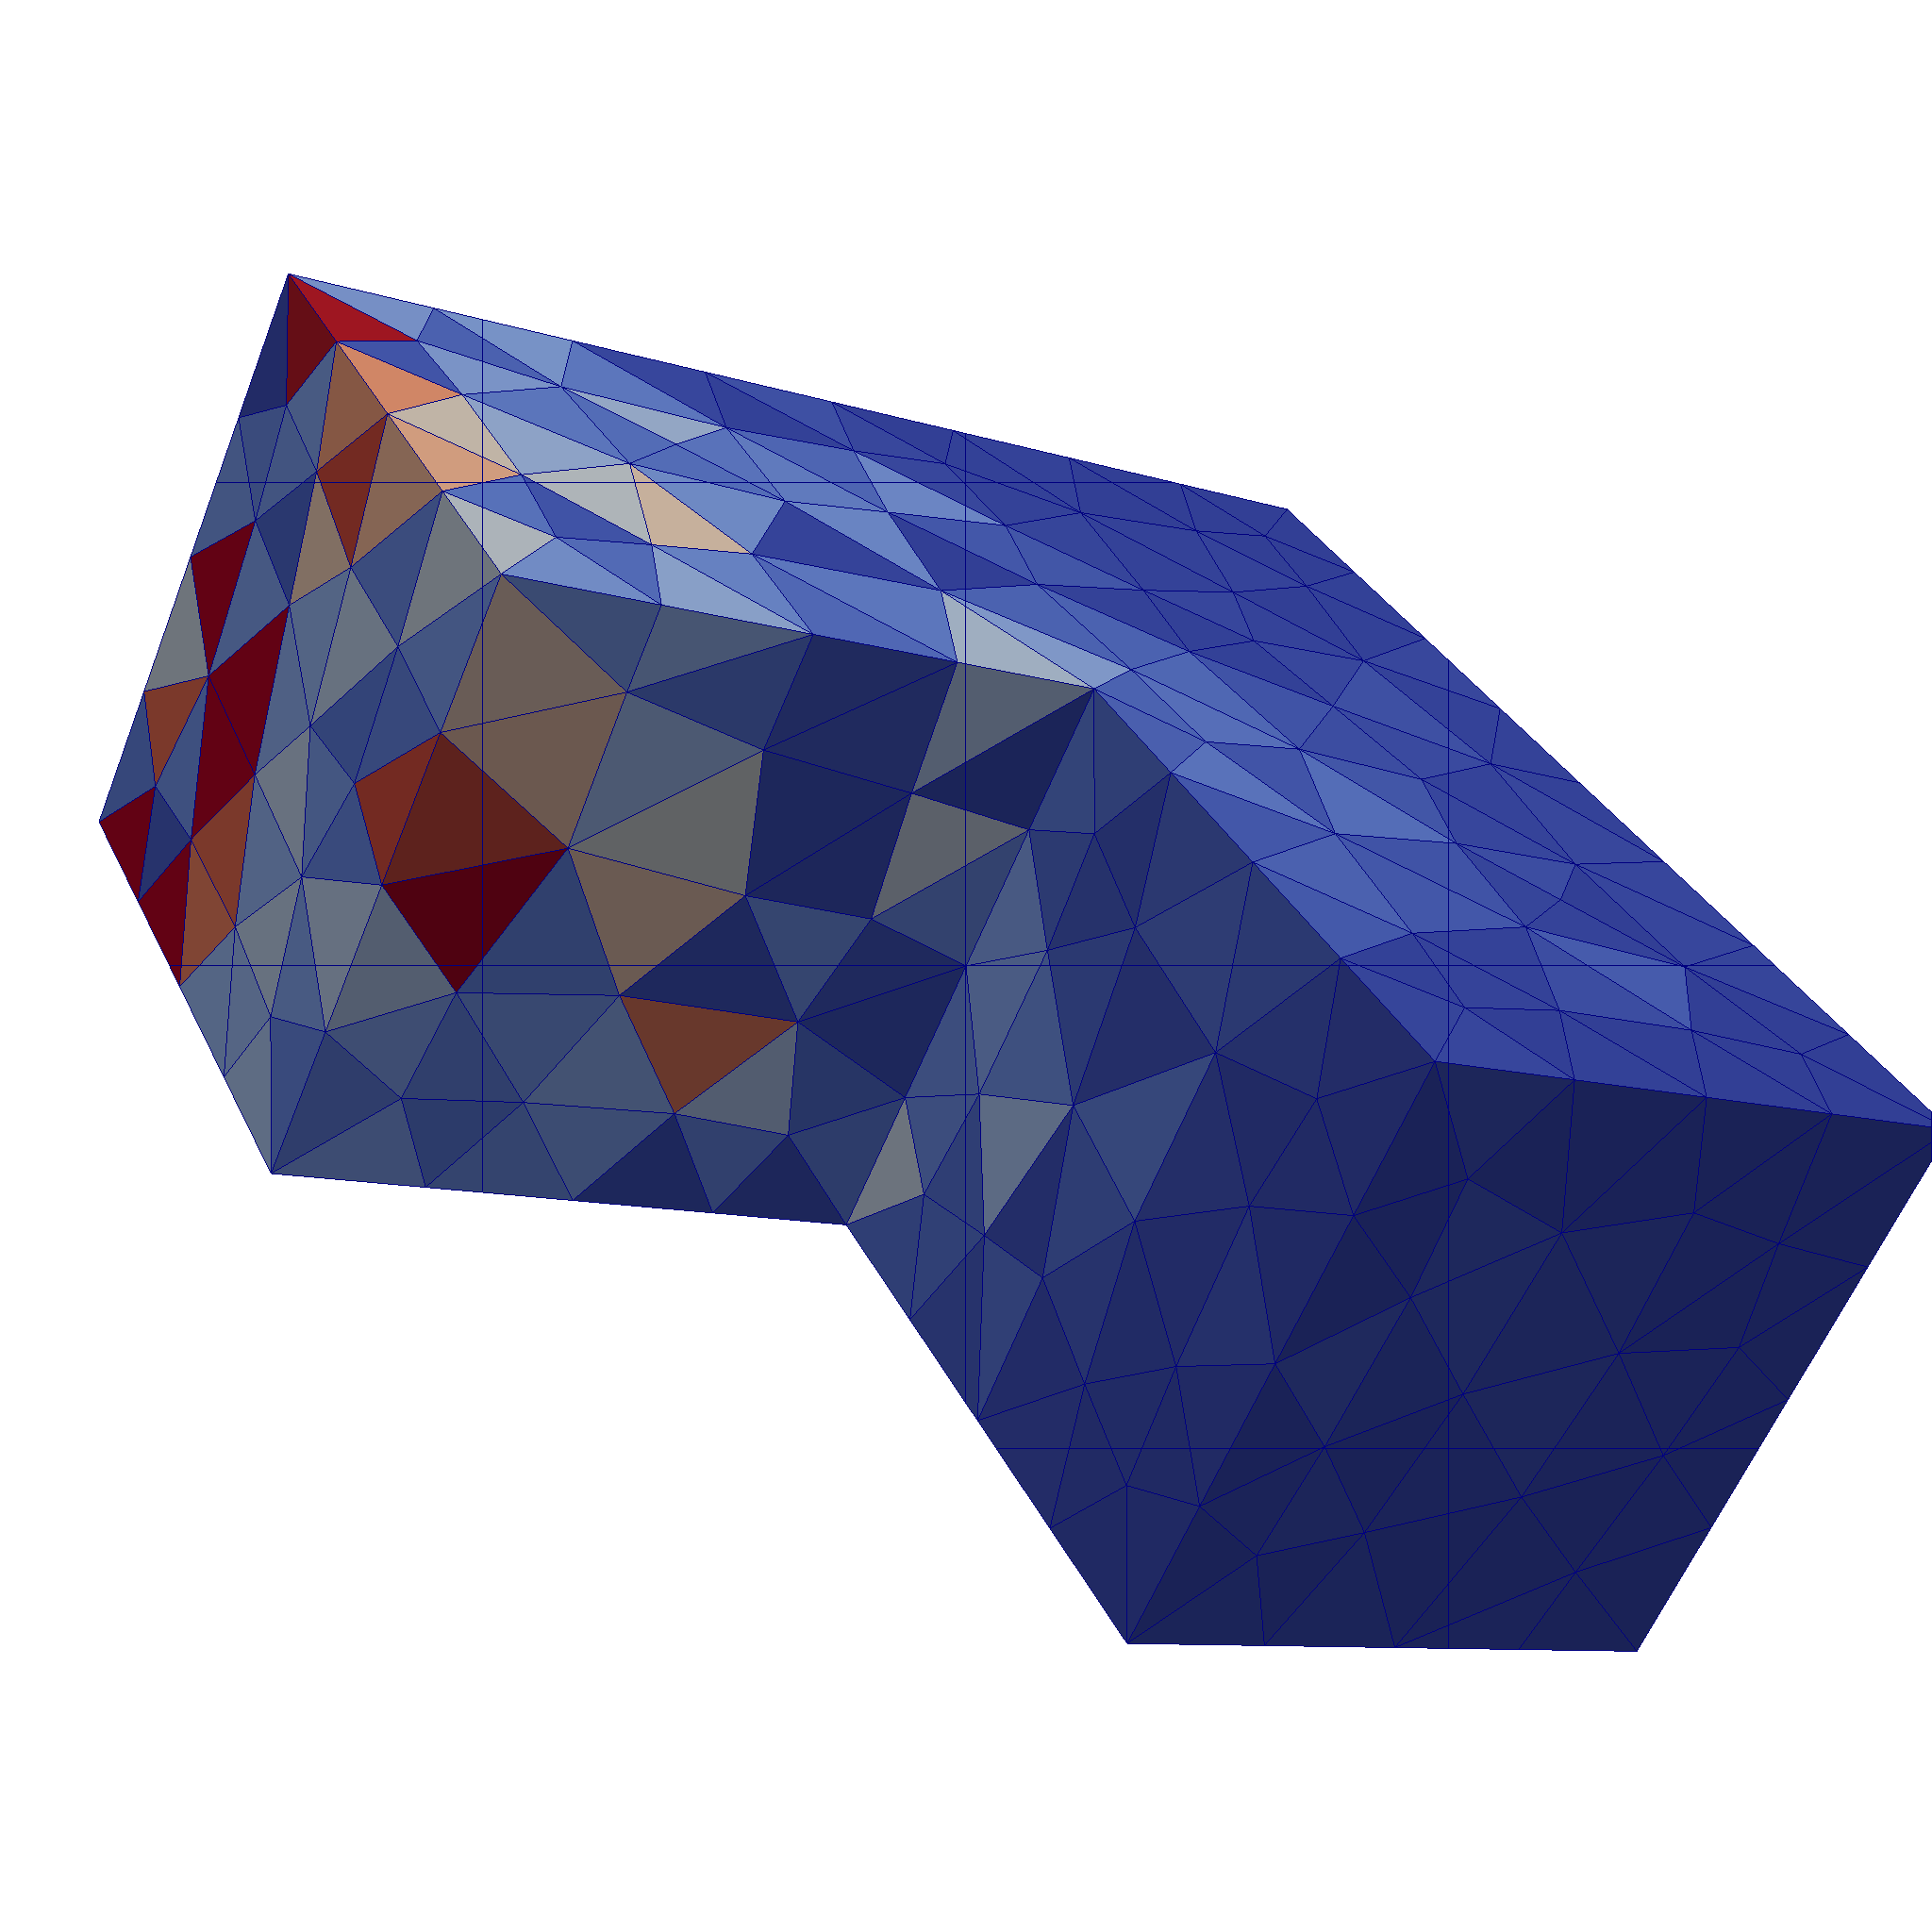
\includegraphics[height=2.5cm]{png/poisson_picture.png}
  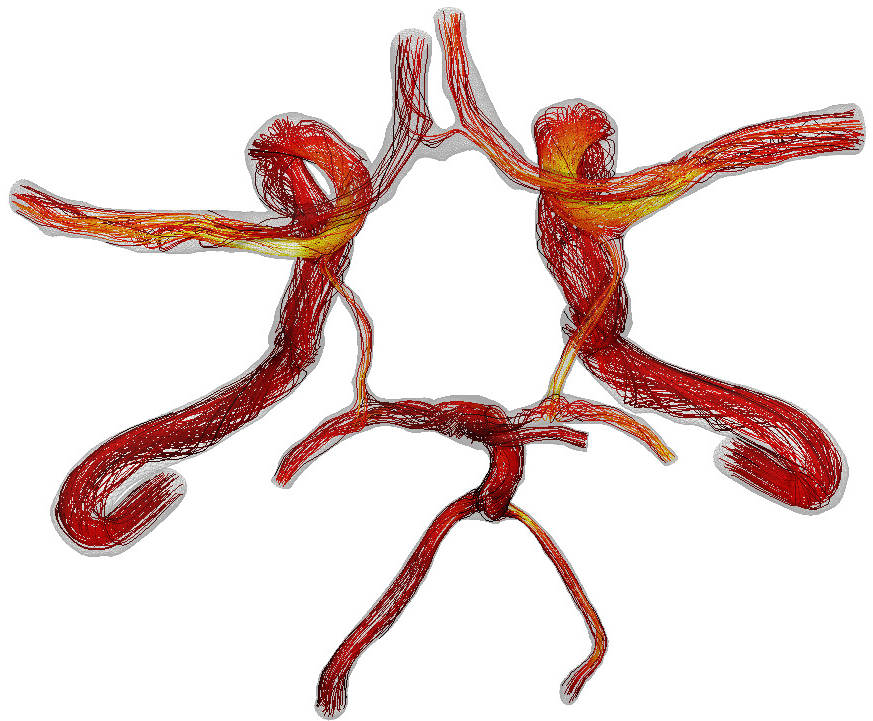
\includegraphics[height=2.5cm]{png/circle_of_willis_simulation.png}
\end{center}

The course gives an introduction to finite element methods and
programming of finite element methods for the solution of a large
selection of partial differential equations, ranging from simple static
linear problems to systems of time-dependent nonlinear problems.
Topics include finite element discretization, higher-order
discretizations, linear and nonlinear problems, saddle-point problems
(the Stokes problem), imcompressible Navier--Stokes equations, static
and dynamic hyperelasticity, discontinuous Galerkin methods, a
posteriori error estimation and adaptivity, optimal control (adjoint
methods), as well as introduction to efficient Python programming for
computational science.

The course will be based on the free/open-source software FEniCS for
automated solution of differential equations in Python (and
C++). FEniCS has a powerful set of features and allows finite element
variational problems to be specified in near-mathematical notation
directly as part of a Python program. For example, the variational
problem for the Poisson equation,
\begin{equation}
  \int_{\Omega} \grad u \cdot \grad v \dx = \int_{\Omega} f v \dx
  \quad \forall v \in V,
\end{equation}
can be directly translated to the following FEniCS program:
\begin{python}
u = TrialFunction(V)
v = TestFunction(V)

a = dot(grad(u), grad(v))*dx
L = f*v*dx
\end{python}
Variational problems like the one above may be solved automatically in
FEniCS:
\begin{python}
u = Function(V)
solve(a == L, u)
\end{python}
Other key features of FEniCS include high-performance linear algebra,
automatic adaptive mesh refinement, postprocessing, and support for a
wide range of finite element function spaces, including high-order
spaces and vector elements.

Participants are expected to have a working knowledge of Python and
basic knowledge of finite element methods. Bring your laptops and be
ready to solve a set of interesting exercises.  Participants are
encouraged to download and install the FEniCS software on their
laptops prior to the course. Participants are also encouraged to
obtain a copy of the FEniCS book. The book and the software are freely
available from the FEniCS Project web site:
\texttt{http://fenicsproject.org/}

\noindent
\begin{minipage}{0.6\textwidth}
  The course will be given by Anders Logg, Professor of Computational
  Mathematics at Chalmers University of Technology, Sweden. Logg is
  co-founder and one of the leading developers of the FEniCS Project.

%  \bigskip
%  The course is organized by C3SE and the Chalmers e-Science Centre.
%  Sign up by email to Stig Larsson \texttt{<stig@chalmers.se>} no later
%  than \textbf{2012--11--30}.
\end{minipage}
\hspace{0.5cm}
\begin{minipage}{0.35\textwidth}
  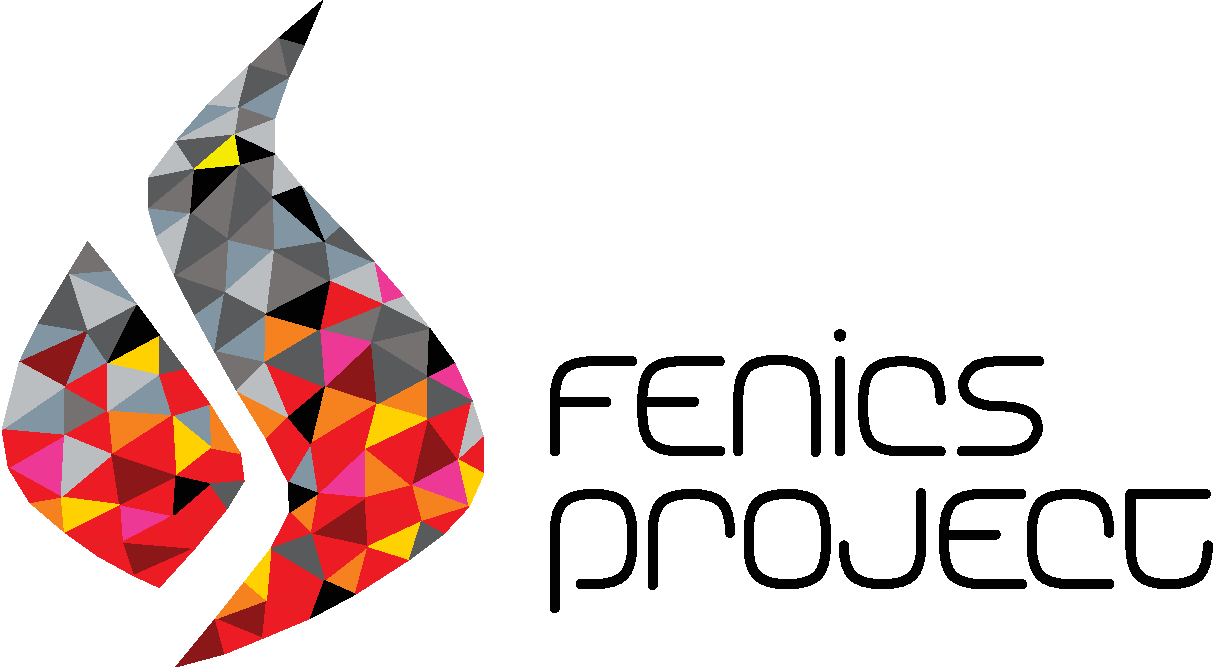
\includegraphics[width=\textwidth]{pdf/fenics_logo_text.pdf}
\end{minipage}
\vspace{0.5cm}

%\noindent
%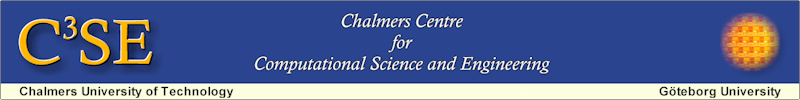
\includegraphics[width=\textwidth]{png/C3SE_stretched.png}

\end{document}
